\chapter{基于Top-K安全混洗的联邦学习模型}
\label{ch4}
\section{引言}
上一章节中所提出的本地自适应差分隐私方案是通过在客户端将梯度上传至参数服务器前,对梯度添加自适应噪声,尽管方案采用了本地差分技术减少一定程度的隐私预算,但Truex等人\upcite{ref49}指出的,一个复杂的隐私保护系统将多个本地差分隐私的算法进行组合,会导致这些算法的隐私成本增长。也就是说,隐私预算为ε1和ε2的本地差分算法的组合会消耗的隐私预算总和为ε1+ε2。使用联邦学习训练的联合模型需要客户在多次迭代中向中央服务器上传梯度更新。如果在迭代训练过程中的每一次迭代都应用本地差分隐私,隐私预算就会累积起来,从而导致总隐私预算的爆炸。在实际的联邦学习应用场景中,本地客户端的数量可能超过千万量级,中央服务器对所有本地上传的加躁梯度进行聚合时,可能因为噪声量的聚合而导致原有的梯度信息被累积的噪声淹没。现有的本地差分隐私协议对于多维聚集的联邦学习框架可能是不可行的,局部噪声带来的误差会随着维度系数的增加而加剧,从而大大降低模型的精度。而且,当参与一次迭代的客户端数量达到千万量级时,会导致聚合任务升级成一个高维任务,隐私预算暴增\upcite{ref43}。在本地设备的模型训练上采用差分隐私技术,对于聚合后的梯度平均估计误差能达到$O\left(\frac{\sqrt{d \log d}}{\epsilon \sqrt{m}}\right)$。

在联邦学习的背景下,传统的经验风险最小化(ERM)存在以下挑战:(i)需要为客户的数据提供隐私保证,(ii)压缩客户和服务器之间的通信,因为客户提供的连接可能为低带宽。提高联邦学习的通信效率分为两种策略,其一,在联邦学习训练期间减少服务器和客户端之间的通信回合数;其二,在每一次服务器和客户端的通信过程中传输更少的参数。现有的研究包括使用静态抽样来选择一部分客户模型参与全局更新,或者对客户端上传的参数使用压缩算法来提高通信效率。

在最近的研究工作中,人们提出了一个新的隐私框架,使用匿名化的方式上传模型参数到中央服务器,即所谓的安全混洗模型(Secure Shuffle Model,SS)。安全混洗是一个针对n个客户和一个中央服务器的隐私保护框架。它使每个客户可以提交一个或多个消息,服务器从所有客户那里了解到一个无序的消息集合,除了本地客户上传的信息,服务器没有能力将任何信息与信息所属的客户联系起来。

安全混洗模型的准确性增益来自于隐私放大效应,对本地设备的输出进行混洗后在差分隐私的中心视图中比没有混洗的输出提供更强的隐私效用。因此,在安全混洗模型中,对于不受信任的中央服务器要达到相同的隐私保护水平,所需要添加的本地噪音更少。然而,目前还不清楚如何在联邦学习中使用SS模型。虽然有一些作品对基本任务进行了研究,如位/实数求和与直方图,但现有的协议对于多维聚合的联邦学习可能是不可行的。

为了应对以上两种挑战,本文根据前人的研究思路,设计了客户端梯度的Top-K采样算法和参数的拆分混洗算法,有效地减少了服务器和客户端的通信过程中传输数据的带宽,提供通信性能的同时也保证了算法整体满足差分隐私。

\section{模型设计}
在安全混洗模型中,我们假设敌手为恶意的第三方服务器和中央服务器,因为它们持有用户本地梯度的所有加密版本。在我们的威胁模型中,我们假设这两种服务器是诚实而好奇的,这意味着每个服务器都诚实地遵守预先商定的程序来完成其任务。然而,它也可能试图通过利用掌握的先验知识来损害用户的数据隐私。此外,我们假设第三方服务器和中央服务器之间不存在串通,混洗器和中央服务器之间不存在串通。

在上述威胁模型下,我们将隐私要求表述如下:
\begin{itemize}
  \item 用户的本地梯度的保密性:敌手如云服务器,可以通过利用共享梯度和全局参数来恢复用户的敏感信息,如数据标签和成员信息。为了保护用户的隐私,每个用户的本地梯度在被发送到服务器之前应该通过安全加密。
  \item 用户所选择的Top-K梯度值对应的索引信息:虽然用户上传的梯度值是添加噪声之后的,但是由于梯度的绝对值和其索引信息是一并发送给混洗器的,本方案需要约束中央服务器成功预测一个索引是否在用户本地向量上传的Top-k元素中。
  \item 对用户的可靠性和聚合结果进行隐私保护:为了使学习过程公平和非歧视性,每个用户的可靠性,即用户的“数据质量”信息,应该被保密,在训练过程中不能被服务器和任何用户获取。另一方面,模型聚合的结果可以被视为有价值的知识产权,它是用大量的资源产生的,甚至包含一些用户的专有信息。因此,除了参与训练的用户之外,聚合的结果对敌手来说应该是保密的。
\end{itemize}

本文基于梯度稀疏化的思想,创造性地开发了Top-k梯度选择算法,应用在安全混洗框架中,与随机扰动相结合,设计了满足$\left(\epsilon_{1}+\epsilon_{2}\right)$-本地差分隐私的算法。在本文,我们将客户端采样和梯度混洗这两种隐私放大效应相结合,实现的方案能提高全局模型的精度,也保证在更低的隐私成本下达到相同的隐私预算,且降低了通信成本,缓解了由维度系数增加而带来的隐私预算暴增和模型精度下降的问题。

我们将在本节详细的描述该框架中各个模块的设计和实现过程。

\subsection{模型概览}
\begin{figure}[!hbt]
\centering
	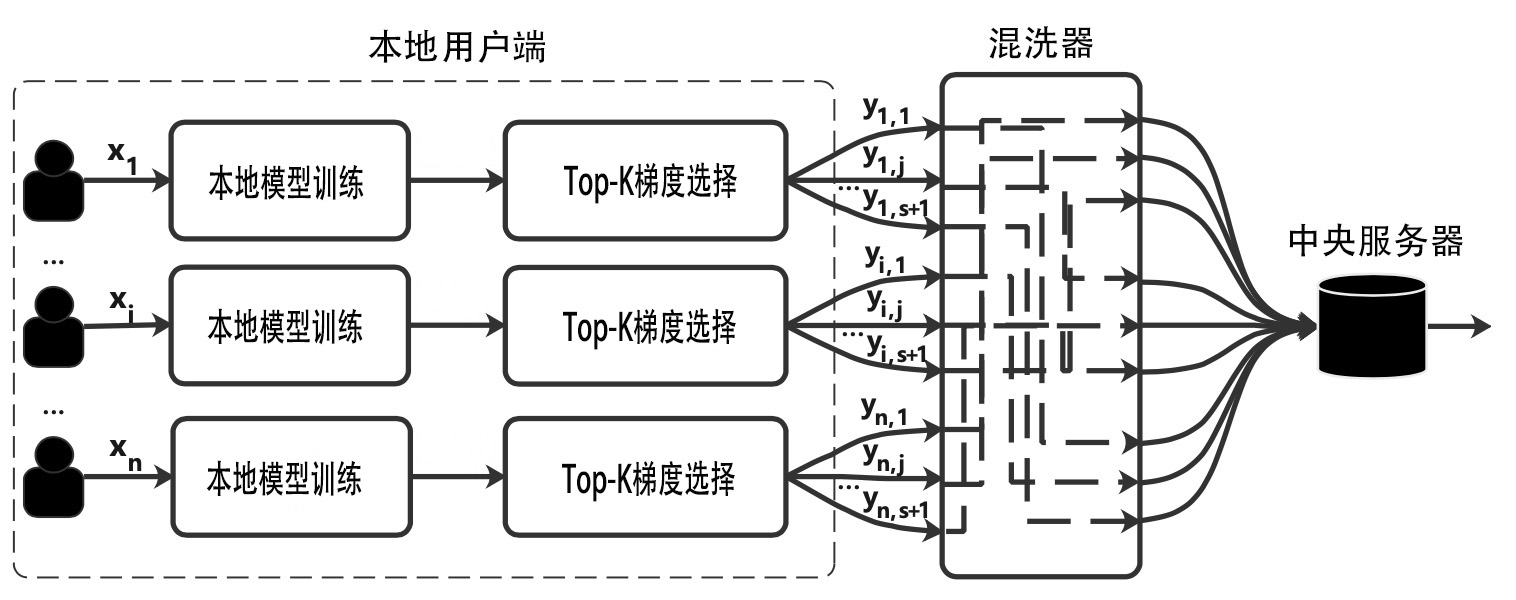
\includegraphics[scale=0.5]{fig2/C4/模型概况图}%联邦学习的系统架构
	\caption{基于安全混洗和Top-K梯度选择算法的联邦学习模型框架}
	\label{fig:基于安全混洗和Top-K梯度选择算法的联邦学习模型框架}	
\end{figure}

如图\ref{fig:基于安全混洗和Top-K梯度选择算法的联邦学习模型框架}所示,该框架主要由本地客户端、混洗器和中央服务器3部分组成:
\begin{itemize}
  \item 本地客户端:本地设备通过模型训练得到梯度向量$\mathbf{g}$,通过Top-K梯度选择算法计算得到满足$\left(\epsilon_{1}+\epsilon_{2}\right)-LDP$的索引列表和梯度元素列表。
  \item 混洗器:对梯度进行拆分混洗,通过隐私放大效应使得算法满足$\epsilon_{0}$-差分隐私,达到梯度匿名机制,最后将混洗后的结果发送至中央服务器。
  \item 中央服务器: 一个诚实但好奇的第三方。服务器接受混洗器上传的梯度并进行聚合,然后更新全局模型。
\end{itemize}

本地客户端在本地进行模型训练后得到梯度向量,根据向量中每一元素的绝对值进行降序排序,以较大的概率选择为top-K元素的梯度值,在梯度上添加拉普拉斯噪声,再以较小的概率选择非top-K元素的梯度值,将得到的索引列表和梯度元素列表上传至安全混洗器。然后安全混洗器将收集到的梯度以维度进行拆分,打乱次序,达到隐私放大效果,再发送给中央服务器进行聚合。安全混洗器独立于服务器并专门用于本地客户端梯度的子采样、拆分混洗、上传。这个模型通过子采样和拆分混洗两者的结合达到隐私放大效应,降低了隐私预算,从而提高了整体联邦学习模型的精度。当本地差分隐私添加更少的噪音时,对于同样的中央服务器能达到相同水平的隐私预算,但通信成本要低得多。

假设现在有m个本地客户端,每个客户端表示为$i \in[m]$,有本地数据集\\$\mathcal{D}_{i}=\left\{d_{i 1}, \ldots, d_{i r}\right\} \in \mathbb{S}^{r}$,由$r$ 个数据集合构成。$F_{i}(\theta)$表示在客户端$i$的本地数据集 $\mathcal{D}_{i}$上进行训练,对于模型梯度$\theta \in \mathbb{R}^{d}$进行衡量的损失函数,其中$F_{i}(\theta)=\frac{1}{r} \sum_{j=1}^{r} f\left(\theta ; d_{i j}\right)$,$f(\theta ; \cdot): \mathcal{C} \rightarrow \mathbb{R}$是凸函数。中央服务器的目标是找到一个最佳的模型参数向量$\theta^{*} \in \mathcal{C}$ 使得损失函数$\min _{\theta \in \mathcal{C}}\left(F(\theta)=\frac{1}{m} \sum_{i=1}^{m} F_{i}(\theta)\right)$最小,其中隐私性满足单个客户端的隐私预算,也就是满足$\epsilon$-差分隐私。

在算法\ref{联邦学习中的安全混洗算法}中,首先我们从m个客户端中随机挑选k个客户端,表示为集合$\mathcal{U}_{t}$,其中$k \leq m$。每个客户端$i \in \mathcal{U}_{t}$从本地数据集中抽样$\mathcal{S}_{i t}$个样本训练模型,计算梯度$\nabla_{\theta_{t}} f\left(\theta_{t} ; d_{i j}\right)$。第$i$个客户端根据Top-K梯度选择算法对梯度进行采样扰动,得到满足$\left(\epsilon_{1}+\epsilon_{2}\right)-LDP$的梯度元素列表和索引列表$\left\langle index_{i,j}, y_{i,j}\right\rangle$。混洗器对收到的梯度$\left\langle y_{i,j} \right\rangle$进行拆分混洗(梯度维度的拆分、输出随机排序的结果),然后发送给中央服务器。最后,中央服务器对混洗后的梯度进行聚合求均值,更新全局模型。

\begin{algorithm}[!htb]
	\caption{联邦学习中的安全混洗算法:$\mathcal{A}_{\text {csdp}}$}
	\label{联邦学习中的安全混洗算法}
	\begin{algorithmic}[1]
		\footnotesize
		\STATE \textbf{输入:} 数据集$\mathcal{D} \quad=\bigcup_{i \in[m]} \mathcal{D}_{i}$, $\mathcal{D}_{i}=\left\{d_{i 1}, \ldots, d_{i r}\right\}$,损失函数 $F(\theta)=$ $\frac{1}{m r} \sum_{i=1}^{m} \sum_{j=1}^{r} f\left(\theta ; d_{i j}\right)$,本地差分隐私预算$\epsilon$,梯度范数阈值$C$,模型学习率$\eta_{t}$,K
		\STATE \textbf{初始化:} $\theta_{0} \in \mathcal{C}$
		\FOR{$t \in[T]$}
			\STATE \textbf{本地更新:}
			\FOR{客户端$i \in \mathcal{U}_{t}$}
				\FOR{样本$j \in \mathcal{S}_{i t}$}
					\STATE $\mathbf{g}_{t}\left(d_{i j}\right) \leftarrow \nabla_{\theta_{t}} f\left(\theta_{t} ; d_{i j}\right)$
					\STATE 梯度裁剪:${\mathbf{g}}_{t}\left(d_{i j}\right) \leftarrow \mathbf{g}_{t}\left(d_{i j}\right) / \max \left\{1, \frac{\left\|\mathbf{g}_{t}\left(d_{i j}\right)\right\|_{p}}{C}\right\}^{3}$
					\STATE Top-K梯度选择:$\left\langle index_{i,j}, y_{i,j}\right\rangle$=Top-k(${\mathbf{g}}_{t}\left(d_{i j}\right)$,K,$\epsilon$)
				\ENDFOR
				\STATE 客户端i将$\left\langle index_{i,j}, y_{i,j}\right\rangle$发送给混洗器
			\ENDFOR
			\STATE \textbf{全局更新:}
			\STATE  混洗器对于$\left\langle index_{i,j}, y_{i,j}\right\rangle$中的权重进行拆分混洗,然后上传给中央服务器
			\STATE 中央服务器聚合梯度:$\overline{\mathbf{g}}_{t} \leftarrow \frac{1}{k s} \sum_{i \in \mathcal{U}_{t}, j \in \mathcal{S}_{i t}} \left\langle y_{i,j} \right\rangle$
			\STATE 梯度下降:$\theta_{t+1} \leftarrow \prod_{\mathcal{C}}\left(\theta_{t}-\eta_{t} \overline{\mathbf{g}}_{t}\right)$
		\ENDFOR
		\STATE \textbf{输出:}最终全局模型参数$\theta_{T}$

	\end{algorithmic}
\end{algorithm}

\newpage

\subsection{Top-K梯度选择算法}
在神经网络的训练过程中,每次迭代的梯度都是从训练样本的小批量子样本中计算得到。直观地说,应用于子样本的算法比应用于全样本的算法具有更强的隐私保证,这种隐私的放大是由于一条数据如果没有在子样本中被选中,就会享有完美的隐私。因此我们在本地用户上传的梯度向量中进行子采样,上传到混洗器。

然而随机子抽样对所有梯度向量的维度一视同仁,因此可能会丢弃“重要”的维度。每个本地客户端从d维的梯度向量中随机采样并扰动k个维度,扰动的值被放大了d/k倍以获得无偏的平均估计,因此注入的噪声也被放大了。对于梯度向量高维的情况(比如,梯度是n维向量,算法从中随机抽取k个维度的梯度值,当n>>k时),从一个向量中随机抽出一小部分β值就会减慢训练的收敛率。根据文献\upcite{ref78}提出的梯度稀疏化技术,作者通过移除梯度向量中绝对值最小的R\%的梯度,使梯度更新算法稀疏化。由于绝对值较小的梯度会随着时间的推移而累积,会破坏模型的收敛性。梯度稀疏化技术通过评判梯度的重要性,仅上传更重要的梯度值而降低通信成本,避免维度爆炸。本文根据梯度稀疏的想法设计了Top-K梯度选择算法,它的主要思想是基于这样一个事实,即具有较大绝对值的梯度可以为模型收敛做出更多贡献,并基于差分隐私选择的技术。

具体来说,算法发生在本地客户端进行随机梯度下降算法得到梯度向量后、将梯度向量上传至混洗器前。首先,本地用户通过SGD算法得到梯度向量$\mathbf{g}$,求得向量中的每一个元素$\mathbf{g}[i]$的绝对值$a b s(\mathbf{g}[i])$,然后根据每一维度的绝对值进行降序排序,得到绝对值最大的K个梯度值。

因为算法的思想是具有较大绝对值的梯度可以为模型收敛做出更多贡献,可以理解为具有最大绝对值的维度应该以最高的概率输出。根据文献\upcite{ref35}提出的指数机制,指数机制是对于任意非数值型的查询,返回最佳的响应,并且满足差分隐私的一种隐私保护机制。指数机制是为以下情况设计的:例如在拍卖中设定价格,目标是使收益最大化,而向最优的价格添加上少量的正噪音(为了保护投标的隐私)会大大减少所产生的收入。对于用户的每个投标价格是需要满足隐私的,但我们又不希望在价格上添加过多的噪音。在本文的场景下,我们希望选择最佳的梯度值,但直接向梯度中添加噪音会完全破坏模型收敛,两个场景的核心问题是相似的。所以首先考虑通过指数机制实现满足差分隐私的top-k梯度选择算法。

在第二章的基础知识中,我们已经介绍了差分隐私中的指数机制。对于一个任意的范围$\mathcal{R}$,通过定义一个实用性函数 $u: \mathbb{N}^{|\mathcal{X}|} \times \mathcal{R} \rightarrow \mathbb{R}$,为用户的数据打分。比如本文中的梯度绝对值越高,那么实用性函数所给的评分也越高。直观地说,用户通过指数机制中的实用性函数能得到给定数据库X中的效用评分最高的数据记录,即top-1数据。实用性函数的敏感度表示为:
$$
\Delta u \equiv \max _{r \in \mathcal{R}} \max _{x, y:\|x-y\|_{1} \leq 1}|u(x, r)-u(y, r)|
$$

对于指数机制$\mathcal{M}_{E}(x, u, \mathcal{R})$,按照正比于$\exp \left(\frac{\varepsilon u(x, r)}{2 \Delta u}\right)$的概率从数据集X中选择,并输出最优元素$r \in \mathcal{R}$,是满足$(\varepsilon, 0)-$差分隐私。

在差分隐私的指数机制中,K值为1,为了适应各种学习任务,K值应该是可调整的,因此本文设计了一种类似于指数机制的扰动采样算法,具体算法流程如图\ref{fig:top-K梯度选择算法流程图}所示。

\begin{figure}[!hbt]
\centering
	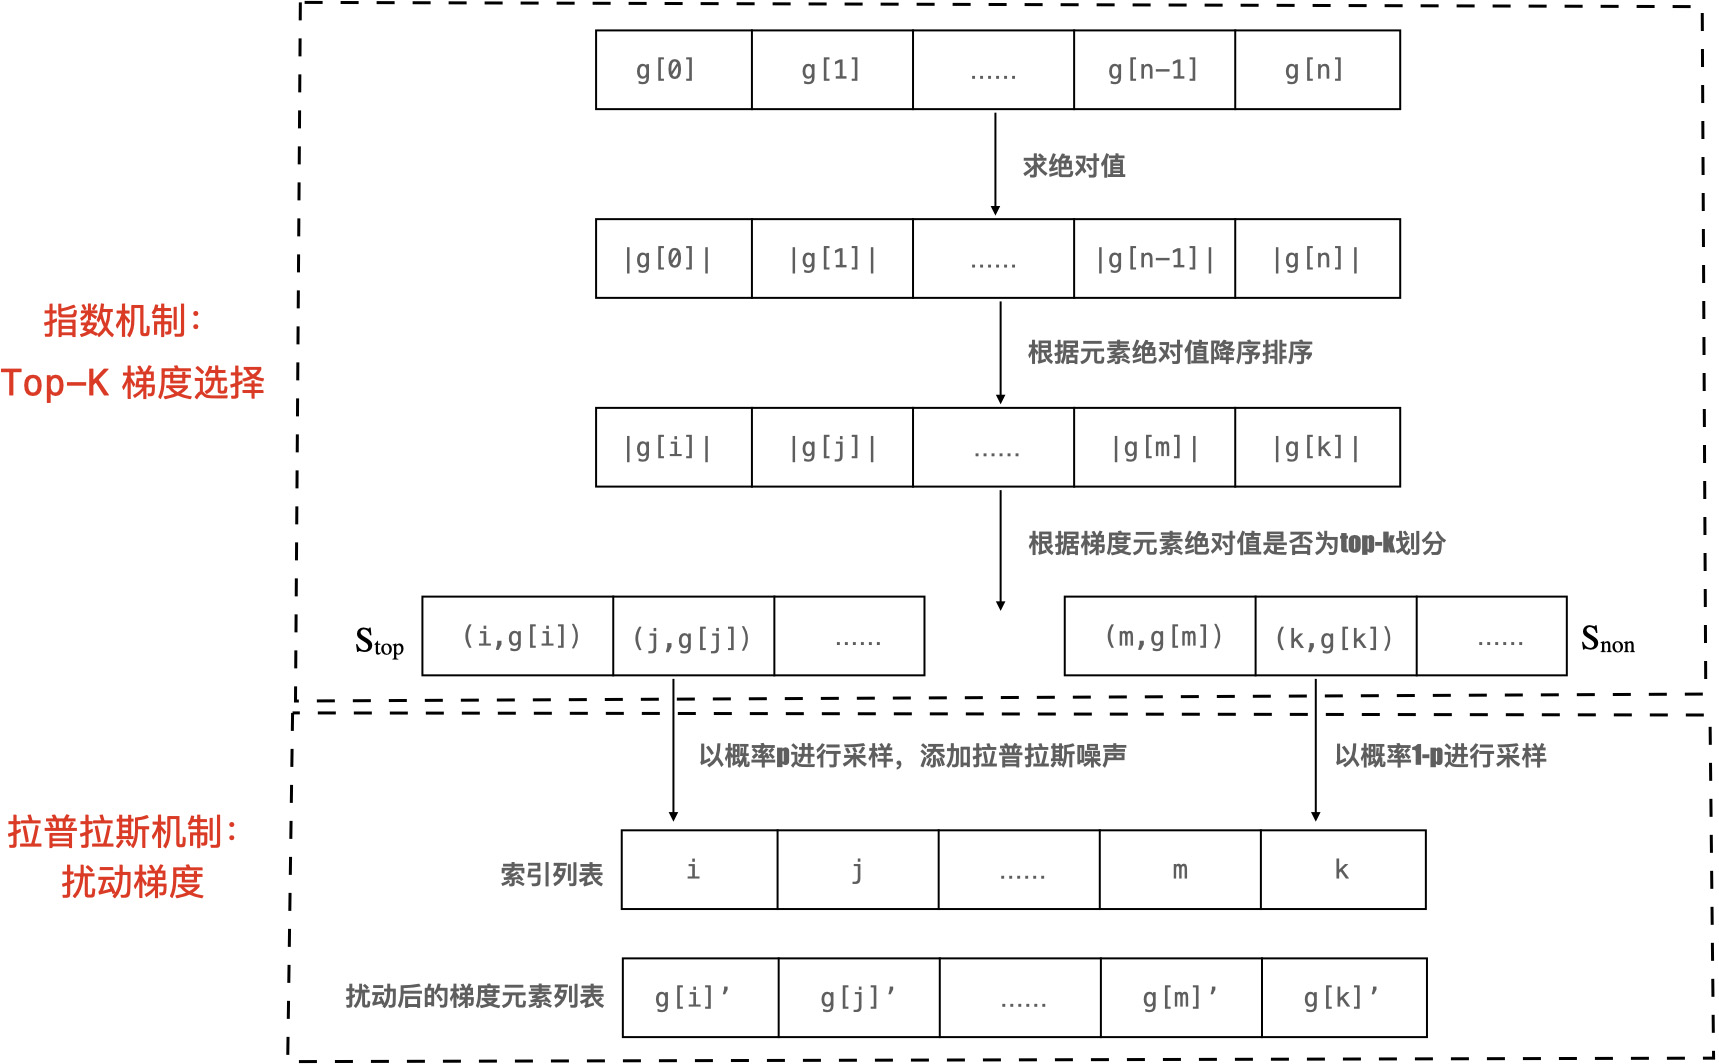
\includegraphics[scale=0.45]{fig2/C4/top-K流程图}%联邦学习的系统架构
	\caption{top-K梯度选择算法流程图}
	\label{fig:top-K梯度选择算法流程图}	
\end{figure}

我们设计了一个二维数组,分别存储梯度值的索引$i$,梯度绝对值$\mathbf{g}[i]$。梯度的置信值$u_{i}$为1或者0,1表示该梯度值属于top-K,0反之。
对于第i个索引的梯度值$\mathbf{g}[i]$,我们将根据其索引对应的梯度置信值进行划分,得到top-K集合$S_{\text {top }} \leftarrow\left\{i \mid i \in \operatorname{Top}\left(\left|\tilde{x}_{i}\right|\right)\right\}$和非top-K集合$S_{\text {non-top}} \leftarrow\left\{i \mid i \in[n] \backslash S_{\text {top }}\right\}$。

\begin{figure}[!hbt]
\centering
	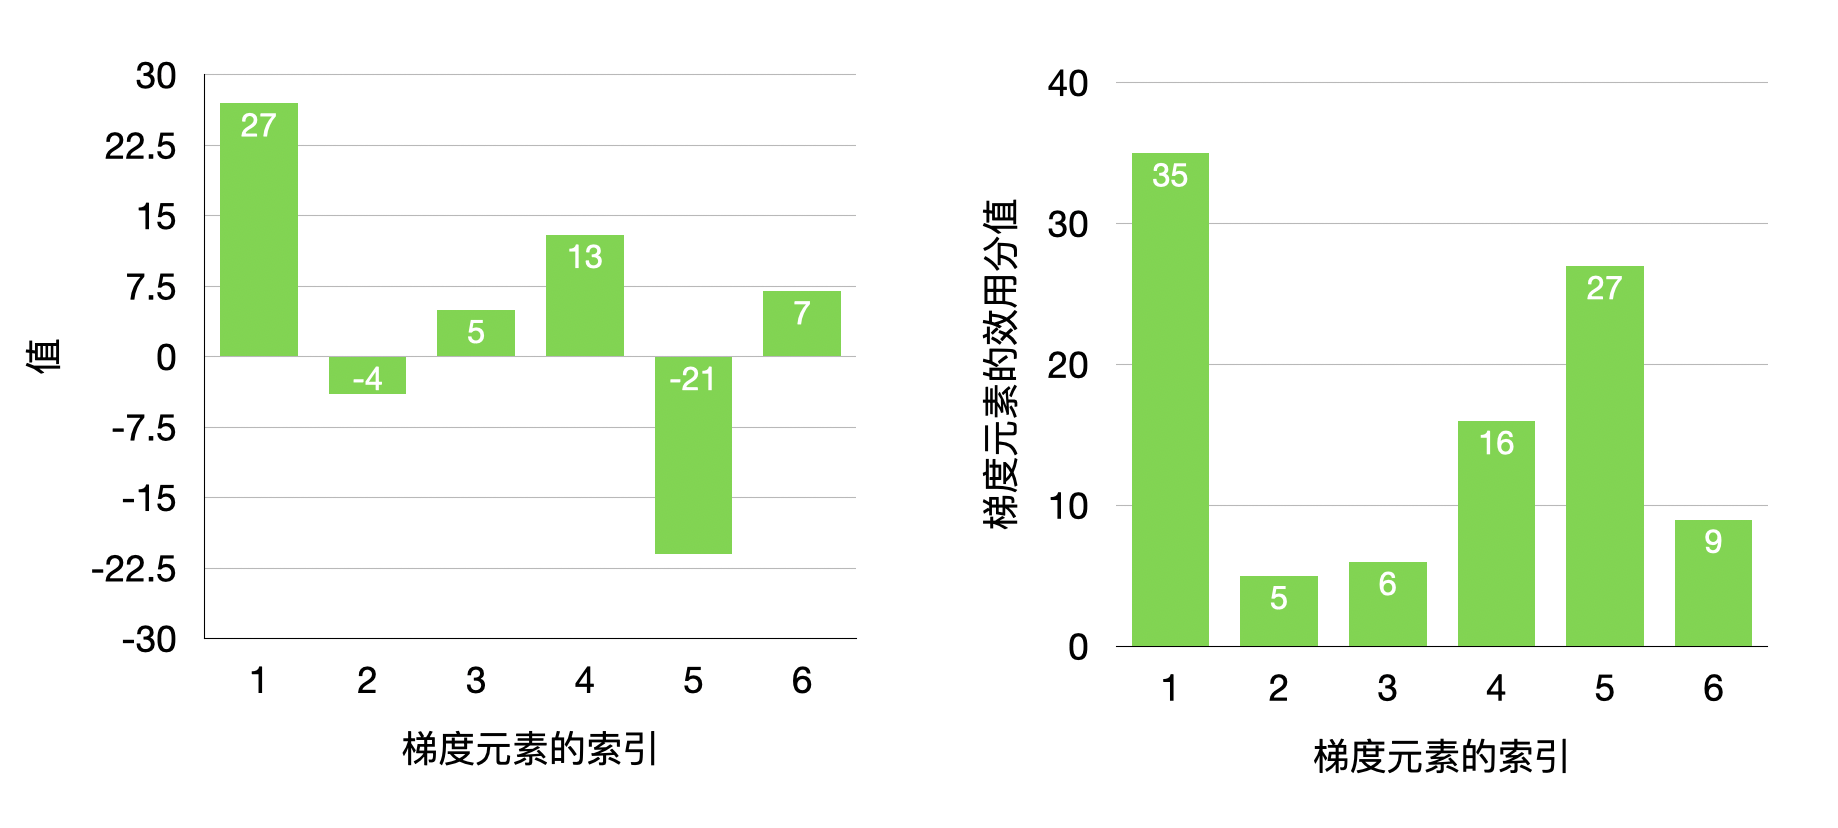
\includegraphics[scale=0.45]{fig2/C4/梯度值打分}%联邦学习的系统架构
	\caption{梯度元素的值及其效用评分}
	\label{fig:梯度元素的值及其效用评分}	
\end{figure}

如图\ref{fig:梯度元素的值及其效用评分}所示,当k=2时,根据梯度元素的绝对值进行降序排序,然后根据其索引对应的梯度值是否为top-k梯度值进行划分,得到,梯度置信向量$u=\left\{u_{1}, \cdots, u_{n}\right\}=\{1,0,0,0,1,0\}$,其中$S_{\text {top }}=\{1,5\}$,$S_{\text {non }}=\{2,3,4\}$。

接着进行概率选择,从n个梯度值构成的数组中以更高的概率p选择属于$S_{\text {top }}$的梯度值$\left\{g[1], \ldots, g[k]\right\} \in\{0,1\}^{k}$,在索引对应的梯度上直接添加拉普拉斯噪声:
$$
g[i]^{\prime}=g[i]+ \operatorname{Lap}\left(\frac{GS_{l}}{\epsilon_{i}}\right)
$$
以较低的概率1-p选择属于$S_{\text {non-top}} $的索引$\left\{g[1], \ldots, g[n-k+1]\right\} \in\{0,1\}^{n-k}$,将采样扰动后的的新的梯度元素及其对应的索引分别存储到两个列表中上传给混洗器,其中,$p=\frac{e^{\epsilon} \cdot k}{n-k+e^{\epsilon} \cdot k}$。这样的概率选择是满足$\epsilon$-差分隐私的,如下给出证明。

\begin{theorem}\label{隐私性证明-topk}
对于给定的梯度分值向量$u, u^{\prime}$,假设算法输出的索引为j,根据条件概率可以给出以下证明:
$$
\frac{\operatorname{Pr}[j \mid u]}{\operatorname{Pr}\left[j \mid u^{\prime}\right]} \leq \frac{\operatorname{Pr}\left[j \mid u_{j}=1\right]}{\operatorname{Pr}\left[j \mid u_{j}^{\prime}=0\right]}=\frac{p \frac{1}{k}}{(1-p) \frac{1}{n-k}}=e^{\epsilon}, \text { where } p=\frac{e^{\epsilon} k}{n-k+e^{\epsilon} \cdot k}.
$$
\end{theorem}

\begin{algorithm}[!htb]
	\caption{Top-K梯度选择算法}
	\label{Top-K梯度选择算法}
	\begin{algorithmic}[1]
		\footnotesize
		\STATE \textbf{输入:} 梯度向量$\mathbf{g}$,K,隐私预算$\epsilon$
		\STATE 初始化:tmp=[],TK=[],$S_{\text {top }}$=[],$S_{\text {non-top}}$=[] ∕∗tmp存储梯度绝对值,TK存储最终输出的梯度元素,$S_{\text {top }}$和$S_{\text {non-top}}$分别存储属于top-k元素的索引值和不属于top-k元素的索引值∗∕
		\FOR{ $\mathbf{g}[i] \in \mathbf{g}$}
			\STATE tmp.append({i,abs($\mathbf{g}[i]$)}); ∕∗tmp中的每个元素分别存储数组的索引和对应的元素绝对值∗∕
		\ENDFOR
		\STATE Sort tmp by tmp.values desc;∕∗根据梯度绝对值对tmp数组进行降序排序∗∕
		\FOR{tmp[i] in tmp}
				\IF{i <k } 
				\STATE $S_{\text {top }}$.append(i);
				\ELSE
				\STATE $S_{\text {non-top }}$.append(i);
				\ENDIF 
		\ENDFOR
		\FOR{each index $i \in S_{\text {top }} \cup S_{\text {non-top}}$}
				\IF{i in $S_{\text {top }}$}
				\STATE $y_{i, j}$=tmp[i].value+ $\operatorname{Lap}\left(\frac{GS_{l}}{\epsilon_{i}}\right)$;
				\ELSE
				\STATE $y_{i, j}$=${\omega_{\mathcal{R}}}_{tmp[i].value}$;
				\ENDIF
		\ENDFOR
		\STATE \textbf{输出:} $\left\langle index_{i}, y_{i}\right\rangle$
	\end{algorithmic}
\end{algorithm}

算法\ref{Top-K梯度选择算法}将满足$\epsilon_{1}-LDP$的梯度选择和满足$\epsilon_{2}-LDP$的拉普拉斯梯度扰动相结合,根据差分隐私的组合定理,整体算法满足$\left(\epsilon_{1}+\epsilon_{2}\right)-LDP$。
接着分析Top-K梯度选择算法的时间复杂度,与非隐私保护的SGD相比,LDP-SGD给本地设备带来了额外的计算成本。对于Top-K梯度选择算法,所有梯度元素的效用分数和总和都可以离线初始化。对一个n维的向量进行排序需要消耗 $O(d \log d)$。将n个维度的元素之映射到相应的效用分数需要消耗$O\left(n^{2}\right)$,元素取样需要$O(n)$。因此,每个本地设备都有额外的时间成本$O\left(n \log n+n^{2}+n\right)=O\left(n^{2}\right)$用于梯度选择和概率选择。由于方案避免了每个维度的梯度扰动,它的计算成本比LDP低很多。

\subsection{拆分混洗算法}
McMahan等人先前的研究工作\upcite{ref52}表明,在联邦学习模型中,假如在某个时间段数据是被适当的匿名化,并将数据之间的耦合信息拆分后,模型整体的隐私保障可以得到极{}大的改善。因此在本章中,我们针对客户端上传的梯度,进行参数的拆分混洗,通过混洗器达到客户端的匿名性,打破从中央服务器接收的数据与特定客户端之间的联系,并在每次迭代中从同一客户端发送的梯度更新中将信息解耦。在安全混洗模型中,利用一个洗牌器来打破用户身份和上传到数据分析器的信息之间的联系。由于需要引入更少的噪音来实现相同的隐私保证,按照这种模式,保护隐私的数据收集的效用得到了改善。

客户端的匿名性可以通过现有的多种机制来实现,这取决于中央服务器在特定场景下如何跟踪客户端。作为一个典型的保护隐私的最佳做法,如果使每个客户对服务器产生一定程度的匿名性,就能使客户的个人身份识别与他们的权重更新无法关联。例如,如果服务器通过IP地址追踪客户,每个客户可以通过使用网络代理、VPN服务、公共WiFi接入产生一个无法追踪的IP地址。再比如,如果服务器通过软件生成的元数据(如ID)来追踪客户,每个客户可以在向服务器发送元数据之前将其随机化。

但是,我们认为,客户端的匿名性不足以防止通信链道的攻击。例如,如果客户端在每次迭代中同时上传了大量的权重更新,中央服务器仍然可以将它们连接在一起。因此,我们设计了混洗算法,以打破来自相同客户的模型权重更新之间的联系,并将其放置于客户端上传梯度更新至中央服务器之间,使中央服务器很难结合多个客户端的同步更新来推断任何本地设备的更多信息,具体算法如\ref{混洗器中的拆分混洗算法}所示。

\begin{algorithm}[!htb]
	\caption{混洗器中的拆分混洗算法}
	\label{混洗器中的拆分混洗算法}
	\begin{algorithmic}[1]
		\footnotesize
		\STATE \textbf{Input:} 本地客户端上传的索引列表和梯度元素列表$\left\langle index_{i,j}, y_{i,j}\right\rangle$
	    \FOR{$(index_{i,j}, y_{i,j}) \in \left\langle index_{i,j}, y_{i,j}\right\rangle$}
	    \STATE 在通信时刻(0,$T$)期间随机采样梯度元素$t_{i d}^{s} \leftarrow U(0, T) \%$
	    \ENDFOR
	    \STATE 在时刻 $t_{i d}^{s}$将梯度元素$(i d, w_{i d})$发送给中央服务器
	\end{algorithmic}
\end{algorithm}

我们的混洗算法通过以下步骤对客户端上传的梯度参数进行混洗,然后上传给中央服务器:
\begin{itemize}
	\item 权重分割:每个客户端都对其本地模型的权重进行分割,但给每个分割后的元素分配一个元数据,以表明其在网络结构中的权重位置。
	\item 权重混洗:对于所有客户端分割后的权重采用随机扰动机制进行混洗。
\end{itemize}

如图\ref{fig:联邦学习安全混洗模型中执行参数拆分混洗的混洗器}所示,假使现有本地模型$X_{1}$,$X_{2}$,$X_{3}$,每个模型都有相同的结构,但权重值不同。原始的联邦学习框架是将模型在本地训练后得到的参数直接发送到中央服务器。图\ref{fig:联邦学习安全混洗模型中执行参数拆分混洗的混洗器}展示了我们的方案中,首先,对于每个模型,我们分割每个本地模型经过本地训练后所产生的权重。然后,对于每个权重,我们通过随机混洗机制对其进行混洗,并将每个权重及其索引发送到中央服务器。

\begin{figure}[!hbt]
\centering
	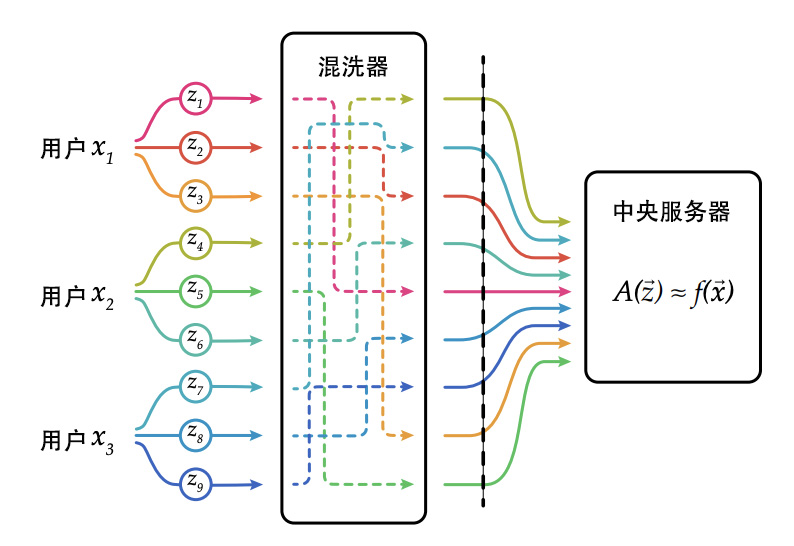
\includegraphics[scale=0.6]{fig2/C4/拆分混洗}%联邦学习的系统架构
	\caption{联邦学习安全混洗模型中执行参数拆分混洗的混洗器}
	\label{fig:联邦学习安全混洗模型中执行参数拆分混洗的混洗器}	
\end{figure}

对于$\epsilon=O(1)$,串行组合的$\epsilon$-LDP算法$\left(A_{1}, \ldots, A_{n}\right)$,令$A_{\text {shuffle }}\left(x_{1}, \ldots, x_{n}\right)=A_{1}\left(x_{\pi(1)}\right), A_{2}\left(x_{\pi(2)}\right), \ldots, A_{n}\left(x_{\pi(n)}\right)$,经过混洗操作$\pi:[n] \rightarrow[n]$后表示为$A_{\text {shuffle }}$,混洗器输出的梯度结果满足$\left(\epsilon^{\prime}, \delta\right)$-DP,其中$\epsilon^{\prime}=O\left(\frac{\epsilon \sqrt{\log (1 / \delta)}}{\sqrt{n}}\right)$。混洗结果并不会改变数据集的统计特性,也不会增加LDP的隐私预算。

\section{隐私性和收敛性证明}
\subsection{隐私性证明}
隐私放大(Privacy Amplification)是本章所提出的安全框架中混洗器对隐私效果增强的理论分析,基于该理论,可将现有的本地化差分隐私方法直接应用在安全框架上。

在算法\ref{联邦学习中的安全混洗算法}中,每个本地客户端采用满足$\left(\epsilon_{1}+\epsilon_{2}\right)-LDP$的Top-K梯度选择算法得到梯度元素列表和索引列表,将其上传至混洗器进行拆分混洗后,所获取的数据满足 $\epsilon_{\mathrm{c}}-\mathrm{DP}$。从 $\left(\epsilon_{c}+\epsilon_{l}\right)$到 $\epsilon_{\mathrm{c}}$ 的转变可通过隐私放大理论证明。$\left(\epsilon_{c}+\epsilon_{l}\right)$ 对应于较大的数值, 表示较低的隐私性; $\epsilon_{\mathrm{c}}$ 对应于较小的数值, 表示较高的隐私性。因此经过混洗器后,隐私性得到了增强。由差分隐私的强组合性可保证Top-K梯度选择算法在每次迭代中对每个样本$d_{i j}$都能保证$\left(\epsilon_{c}+\epsilon_{l}\right)$-本地差异隐私,因此本节只需要分析采样和混洗操作的隐私放大性。

\begin{theorem}\label{隐私性证明}
算法\ref{联邦学习中的安全混洗算法}是满足$(\epsilon, \delta)-$差分隐私的,当对于任意$\delta$,$\delta>0$ ,并且有:
$$
\epsilon=\mathcal{O}\left(\epsilon_{0} \sqrt{\frac{q T \log (2 q T / \delta) \log (2 / \delta)}{n}}\right)
$$
\end{theorem}

假设在联邦学习模型中,需要迭代的次数为$t \in[T]$。$\mathcal{M}_{t}\left(\theta_{t}, \mathcal{D}\right)$表示在时刻$t$对于数据集$\mathcal{D}$和模型参数为$\theta_{t}$的差分隐私机制,$\theta_{t+1}$表示模型的输出。因此,在数据集$\mathcal{D}=\bigcup_{i=1}^{m} \mathcal{D}_{i} \in \mathfrak{S}^{n}$上的差分隐私机制定义如下:

\begin{equation}\label{eq:隐私性证明机制}
\mathcal{M}_{t}\left(\theta_{t} ; \mathcal{D}\right)=\mathcal{H}_{k s} \circ \operatorname{samp}_{m, k}\left(\mathcal{G}_{1}, \ldots, \mathcal{G}_{m}\right)
\end{equation}

其中,$\mathcal{G}_{i}=\operatorname{samp}_{r, s}\left(\mathcal{R}\left(\boldsymbol{x}_{i 1}^{t}\right), \ldots, \mathcal{R}\left(\boldsymbol{x}_{i r}^{t}\right)\right)$并且$\boldsymbol{x}_{i j}^{t}=$$\nabla_{\theta_{t}} f\left(\theta_{t} ; d_{i j}\right), \forall i \in[m], j \in[r]$。$\mathcal{H}_{k s}$表示在$k s$个数据样本上进行混洗操作, $\operatorname{samp}_{a, b}$表示从有a个元素的集合中随机抽样b个元素的操作,$\mathcal{R}\left(\boldsymbol{x}_{i 1}^{t}\right)$表示本地客户端采用Top-K梯度选择算法得到满足$\left(\epsilon_{1}+\epsilon_{2}\right)-LDP$的梯度向量。

接下来我们给出$\mathcal{M}_{t}$的隐私性证明:

假设客户端$i \in[m]$的本地数据集为$\mathcal{D}_{i}=\left\{d_{i 1}, d_{i 2}, \ldots, d_{i r}\right\} \in \mathfrak{S}^{r}$,$\mathcal{D}=\bigcup_{i=1}^{m} \mathcal{D}_{i}$表示总体数据集。根据公式\ref{eq:隐私性证明机制},$\mathcal{Z}\left(\mathcal{D}^{(t)}\right)=\mathcal{H}_{k s}\left(\mathcal{R}\left(\boldsymbol{x}_{1}^{t}\right), \ldots, \mathcal{R}\left(\boldsymbol{x}_{k s}^{t}\right)\right)$表示在本地客户端进行模型训练得到满足本地差分隐私的$ks$个权重集合上混洗后的权重。任取$\tilde{\delta}>0$,当$\epsilon_{0} \leq \frac{\log (k s / \log (1 / \tilde{\delta}))}{2}$时,算法$\mathcal{Z}$ 满足 $(\tilde{\epsilon}, \tilde{\delta})-\mathrm{DP}$差分隐私,可得:

\begin{equation}\label{eq:隐私性证明机制2}
\tilde{\epsilon}=\mathcal{O}\left(\min \left\{\epsilon_{0}, 1\right\} e^{\epsilon_{0}} \sqrt{\frac{\log (1 / \tilde{\delta})}{k s}}\right)
\end{equation}

当$\epsilon_{0}=\mathcal{O}(1)$时,有$\tilde{\epsilon}=\mathcal{O}\left(\epsilon_{0} \sqrt{\frac{\log (1 / \tilde{\delta})}{k s}}\right)$。

令$\mathcal{T} \subseteq\{1, \ldots, m\}$表示在时刻$t$选取的k个客户端。对于$i \in \mathcal{T}$,$\mathcal{T}_{i} \subseteq\{1, \ldots, r\}$表示在时刻$t$客户端$i$所抽样的$s$条数据样本。对于任意的 $\mathcal{T} \in\left(\begin{array}{c}{[m]} \\ k\end{array}\right)$和$\mathcal{T}_{i} \in\left(\begin{array}{c}{[r]} \\ s\end{array}\right), i \in \mathcal{T}$,有$\overline{\mathcal{T}}=\left(\mathcal{T}, \mathcal{T}_{i}, i \in \mathcal{T}\right), \mathcal{D}^{\mathcal{T}_{i}}=\left\{d_{j}: j \in \mathcal{T}_{i}\right\}$ for $i \in \mathcal{T}$, and $\mathcal{D}^{\bar{\top}}=\left\{\mathcal{D}^{\mathcal{T}_{i}}: i \in \mathcal{T}\right\}$。$\mathcal{T}$和$\mathcal{T}_{i}, i \in \mathcal{T}$为抽样产生的任意子集,其中的随机性由客户端抽样和数据集抽样所决定。算法$\mathcal{M}_{t}$可以等价的表示为$\mathcal{M}_{t}=\mathcal{Z}\left(\mathcal{D}^{\overline{\mathcal{T}}}\right)$。

假设现有数据集:$\mathcal{D}^{\prime}=\left(\mathcal{D}_{1}^{\prime}\right) \bigcup\left(\cup_{i=2}^{m} \mathcal{D}_{i}\right) \in \mathfrak{S}^{n}$,其中数据集$\mathcal{D}_{1}^{\prime}=\left\{d_{11}^{\prime}, d_{12}, \ldots, d_{1 r}\right\}$和$\mathcal{D}_{1}$ 为相邻数据集,它们的第$d_{11}$条和第$d_{11}^{\prime}$条数据样本不同。如果$\mathcal{M}_{t}$是满足$(\bar{\epsilon}, \bar{\delta})-\mathrm{DP}$差分隐私的,那么对于算法$\mathcal{M}_{t}$所选的任意子集$\mathcal{S}$ 都应该满足:
\begin{equation}\label{eq:隐私性证明3}
\operatorname{Pr}\left[\mathcal{M}_{t}(\mathcal{D}) \in \mathcal{S}\right] \leq e^{\bar{\epsilon}} \operatorname{Pr}\left[\mathcal{M}_{t}\left(\mathcal{D}^{\prime}\right) \in \mathcal{S}\right]+\bar{\delta}
\end{equation}

\begin{equation}\label{eq:隐私性证明4}
\operatorname{Pr}\left[\mathcal{M}_{t}\left(\mathcal{D}^{\prime}\right) \in \mathcal{S}\right] \leq e^{\bar{\epsilon}} \operatorname{Pr}\left[\mathcal{M}_{t}(\mathcal{D}) \in \mathcal{S}\right]+\bar{\delta}
\end{equation}

由于式\ref{eq:隐私性证明3}和\ref{eq:隐私性证明4}是对称的,因此只需要证明其中一条。下文给出式\ref{eq:隐私性证明3}的证明:

令$q=\frac{k s}{m r}$,我们给出条件概率的定义:
\begin{equation}\label{eq:隐私性证明5}
\begin{array}{l}
A_{11}=\operatorname{Pr}\left[\mathcal{Z}\left(\mathcal{D}^{\overline{\mathcal{T}}}\right) \in \mathcal{S} \mid 1 \in \mathcal{T} \text { and } 1 \in \mathcal{T}_{1}\right] \\
A_{11}^{\prime}=\operatorname{Pr}\left[\mathcal{Z}\left(\mathcal{D}^{\prime} \overline{\mathcal{T}}\right) \in \mathcal{S} \mid 1 \in \mathcal{T} \text { and } 1 \in \mathcal{T}_{1}\right] \\
A_{10}=\operatorname{Pr}\left[\mathcal{Z}\left(\mathcal{D}^{\overline{\mathcal{T}}}\right) \in \mathcal{S} \mid 1 \in \mathcal{T} \text { and } 1 \notin \mathcal{T}_{1}\right]=\operatorname{Pr}\left[\mathcal{Z}\left(\mathcal{D}^{\prime \overline{\mathcal{T}}}\right) \in \mathcal{S} \mid 1 \in \mathcal{T} \text { and } 1 \notin \mathcal{T}_{1}\right] \\
A_{0}=\operatorname{Pr}\left[\mathcal{Z}\left(\mathcal{D}^{\bar{T}}\right) \in \mathcal{S} \mid 1 \notin \mathcal{T}\right]=\operatorname{Pr}\left[\mathcal{Z}\left(\mathcal{D}^{\prime \bar{\tau}}\right) \in \mathcal{S} \mid 1 \notin \mathcal{T}\right]
\end{array}
\end{equation}

令$q_{1}=\frac{k}{m}$,$q_{2}=\frac{s}{r}$,那么$q=q_{1} q_{2}$,然后可以得到:
\begin{equation}\label{eq:隐私性证明6}
\begin{aligned} 
\operatorname{Pr}\left[\mathcal{M}_{t}(\mathcal{D}) \in \mathcal{S}\right] &=q A_{11}+q_{1}\left(1-q_{2}\right) A_{10}+\left(1-q_{1}\right) A_{0}
\end{aligned}
\end{equation}

\begin{equation}\label{eq:隐私性证明7}
\begin{aligned} 
\operatorname{Pr}\left[\mathcal{M}_{t}\left(\mathcal{D}^{\prime}\right) \in \mathcal{S}\right] &=q A_{11}^{\prime}+q_{1}\left(1-q_{2}\right) A_{10}+\left(1-q_{1}\right) A_{0} 
\end{aligned}
\end{equation}

因此,我们可以得到:
\begin{equation}\label{隐私性证明8}
A_{11} \leq e^{\tilde{\epsilon}} A_{11}^{\prime}+\tilde{\delta}
\end{equation}

\begin{equation}\label{隐私性证明9}
A_{11} \leq e^{\tilde{\epsilon}} A_{10}+\tilde{\delta}
\end{equation}
式\ref{eq:隐私性证明7}成立,因此混洗器$\mathcal{M}_{t}$是满足$\varepsilon_{\mathrm{c}}$-差分隐私的。

\subsection{模型收敛性分析}
在本节中,我们分析采用采样和混洗算法后模型的收敛性。

回顾第二章的基础知识,在随机梯度下降算法的每次迭代中,中央服务器将当前的参数向量发送给所有本地客户端,客户端收到后在本地数据集上进行模型训练,计算本地模型的梯度并上传给中央服务器,然后中央服务器计算收到的梯度的平均值/平均数并更新全局模型。

在算法\ref{联邦学习中的安全混洗算法}中,在每一轮迭代过程中,中央服务器聚合上传的$ks$个加躁后的梯度,如算法\ref{联邦学习中的安全混洗算法}的第15行所示,中央服务器进行聚合后得到结果:$\overline{\mathbf{g}}_{t} \leftarrow \frac{1}{k s} \sum_{i \in \mathcal{U}_{t}, j \in \mathcal{S}_{i t}} \left\langle y_{i,j} \right\rangle$,然后通过随机梯度下降算法更新全局模型参数:$\theta_{t+1} \leftarrow \prod_{\mathcal{C}}\left(\theta_{t}-\eta_{t} \overline{\mathbf{g}}_{t}\right)$。

既然随机扰动机制是无偏的,那么平均梯度$\overline{\mathbf{g}}_{t}$也是无偏的,也就是说,我们有 $\mathbb{E}\left[\overline{\mathbf{g}}_{t}\right]=\nabla_{\theta_{t}} F\left(\theta_{t}\right)$,其中期望是相对于客户端和数据点的随机抽样以及扰动机制的随机性而言的。

令$F(\theta)$为凸函数,考虑这样一个随机梯度下降算法:$\theta_{t+1} \leftarrow \prod_{\mathcal{C}}\left(\theta_{t}-\eta_{t} \mathbf{g}_{t}\right)$,$\mathbf{g}_{t}$满足$\mathbb{E}\left[\mathbf{g}_{t}\right]=\nabla_{\theta_{t}} F\left(\theta_{t}\right)$并且$\mathbb{E}\left\|\mathbf{g}_{t}\right\|_{2}^{2} \leq G^{2}$。当确定$\eta_{t}=\frac{D}{G \sqrt{t}}$,可以得到:
\begin{equation}\label{eq:模型收敛性证明1}
\mathbb{E}\left[F\left(\theta_{T}\right)\right]-F\left(\theta^{*}\right) \leq 2 D G \frac{2+\log (T)}{\sqrt{T}}=\mathcal{O}\left(D G \frac{\log (T)}{\sqrt{T}}\right)
\end{equation} 

由Nesterov等人在文献\upcite{ref50}中的证明可知,算法\ref{联邦学习中的安全混洗算法}的输出$\theta_{T}$满足:
\begin{equation}\label{eq:模型收敛性证明2}
\mathbb{E}\left[F\left(\theta_{T}\right)\right]-F\left(\theta^{*}\right) \leq \mathcal{O}\left(\frac{L D \log (T) \max \left\{d^{\frac{1}{2}-\frac{1}{p}}, 1\right\}}{\sqrt{T}}\left(1+\sqrt{\frac{c d}{q n}}\left(\frac{e^{\epsilon_{0}}+1}{e^{\epsilon_{0}}-1}\right)\right)\right)
\end{equation}

其中,存在$\sqrt{1+\frac{c d}{q n}\left(\frac{e^{\epsilon_{0}}+1}{e^{\epsilon_{0}}-1}\right)^{2}} \leq\left(1+\sqrt{\frac{c d}{q n}}\left(\frac{e^{\epsilon_{0}}+1}{e^{\epsilon_{0}-1}}\right)\right)$。

当$\sqrt{\frac{c d}{q n}}\left(\frac{e^{\epsilon_{0}}+1}{e^{\epsilon_{0}}-1}\right) \geq \Omega(1)$时,可以推导出:
\begin{equation}\label{eq:模型收敛性证明3}
\mathbb{E}\left[F\left(\theta_{T}\right)\right]-F\left(\theta^{*}\right) \leq \mathcal{O}\left(\frac{L D \log (T) \max \left\{d^{\frac{1}{2}-\frac{1}{p}}, 1\right\}}{\sqrt{T}} \sqrt{\frac{c d}{q n}}\left(\frac{e^{\epsilon_{0}}+1}{e^{\epsilon_{0}}-1}\right)\right)
\end{equation}

如果我们在算法\ref{联邦学习中的安全混洗算法}中设置学习率为$\eta_{t}=\frac{D}{G \sqrt{t}}$,其中\\$G^{2}=$ $L^{2} \max \left\{d^{1-\frac{2}{p}}, 1\right\}\left(1+\frac{c d}{q n}\left(\frac{e^{\epsilon_{0}}+1}{e^{\epsilon_{0}-1}}\right)^{2}\right)$。那么:

\begin{equation}\label{eq:模型收敛性证明4}
\mathbb{E}\left[F\left(\theta_{T}\right)\right]-F\left(\theta^{*}\right) \leq \\
\mathcal{O}\left(\frac{L D \log (T) \max \left\{d^{\frac{1}{2}-\frac{1}{p}}, 1\right\}}{\sqrt{T}} \sqrt{\frac{c d}{q n}}\left(\frac{e^{\epsilon_{0}}+1}{e^{\epsilon_{0}}-1}\right)\right)
\end{equation}

其中,当$p \in\{1, \infty\}$时,$c=4$否则$c=14$。

\begin{theorem}[随机梯度下降算法的收敛性]\label{随机梯度下降算法的收敛性}
假使有凸函数$F(\theta)$,数据集$D$的维度为$\mathcal{C}$,在模型训练过程中采用随机梯度下降算法$\theta_{t+1} \leftarrow \prod_{\mathcal{C}}\left(\theta_{t}-\eta_{t} \mathbf{g}_{t}\right)$,其中 $\mathbf{g}_{t}$满足$\mathbb{E}\left[\mathbf{g}_{t}\right]=\nabla_{\theta_{t}} F\left(\theta_{t}\right)$并且$\mathbb{E}\left\|\mathbf{g}_{t}\right\|_{2}^{2} \leq G^{2}$。当$\eta_{t}=$ $\frac{D}{G \sqrt{t}}$,$\mathbb{E}\left[F\left(\theta_{T}\right)\right]-F\left(\theta^{*}\right) \leq 2 D G\left(\frac{2+\log (T)}{\sqrt{T}}\right)$成立。
\end{theorem}

根据文献\upcite{ref50}中已有的标准随机梯度下降算法收敛结果中使用的定理\ref{随机梯度下降算法的收敛性}对$G^{2}$的约束条件,证明了混洗算法可在$G^{2}=$ $L^{2} \max \left\{d^{1-\frac{2}{p}}, 1\right\}\left(1+\frac{c d}{q n}\left(\frac{e^{\epsilon}+1}{e^{\epsilon-1}}\right)^{2}\right)$时达到全局最优解。

\section{实验评估}
\subsection{实验准备}
在本节中,我们进行实验来评估混洗器的性能。所有的实验都是用PYTHON语言编译的,其中每个用户都由配备6GB内存、四核2.36GHz Cortex A73处理器和四核Cortex A53 1.8GHz处理器的华为nova3安卓手机代替。中央服务器是用两台联想服务器模拟的,这两台服务器有2个英特尔(R)至强(R)E5-2620 2.10GHZ CPU,32GB内存,512SSD,2TB机械硬盘,运行于Ubuntu 18.04操作系统。

在实验过程中,我们选择了深度学习中常用的两个经典数据集--MNIST手写体数字识别数据集、FMNIST和CIFAR-10数据集进行实验,评估所提出的安全混洗框架。此外,我们让所有用户离线训练一个统一的卷积神经网络,以获得本地用户的梯度。在我们的实验中采用的模型网络结构为CNN,包括2个卷积层,两个池化层层和一个全连接层(32个神经元)。模型的激活函数为Softmax,并引入了DropOut正则以提高模型的泛化能力。下表展示了CNN的网络结构。

\begin{table}[H]
	\centering
	\begin{tabular}{cc}
		\hline
		神经层& 参数\\
		\hline
		卷积层& 8 × 8的16个滤波器,步长为2\\
		池化层& 2 × 2\\
		卷积层& 4 × 4的32个滤波器,步长为2\\
		池化层& 2 × 2\\
		全连接层& 32个神经元\\
		Softmax& 10个神经元\\
		\hline
	\end{tabular}
	\caption{安全混洗框架实验的模型网络结构}
	\label{tab1}
\end{table}

\subsection{实验设计}
在我们模拟的联邦学习环境中,我们设置本地客户端的总数为1000个,其中每个客户有一个本地数据集,每个客户都对梯度$\mathbf{g}_{t}\left(d_{i j}\right) \leftarrow \nabla_{\theta_{t}} f\left(\theta_{t} ; d_{i j}\right)$进行剪裁,梯度裁剪参数C=1/100。之后,运行Top-K梯度选择和拆分混洗算法,混洗器将参数上传至中央服务器进行安全聚合,更新全局参数。我们的算法运行了100个历时,在前80个历时中,我们将学习率设置为0.3,在剩余的历时中,将其降低到0.18。在每一次训练迭代过程中,本地客户端与混洗器、中央服务器进行交互计算得到安全聚合之后的全局梯度向量。我们设置了本地隐私参数$\sigma$=2,而中央隐私参数$\epsilon$的计算则是由我们来完成的。我们首先使用文献中\upcite{ref72}的定理5.3通过洗牌数值计算隐私放大率。然后,我们通过\ref{隐私性证明}中提出的子抽样计算隐私放大;最后,我们使用差分隐私的强组合性质来获得中央隐私参数$\epsilon$。

我们的实验主要分为两个部分:
\begin{enumerate}
\item [(1)] 在MNIST、FMNIST和CIFAR上评估安全混洗算法,评估参数:客户端数量$N$、梯度选择的比率、客户端采样比$f_{r}$和最大聚合次数对于模型分类准确率的影响。
\item [(2)] 将本文的安全混洗方案与基准方案(非隐私保护的联邦学习方案)、前人提出的隐私保护联邦学习方案(如表\ref{tab1}所示)进行对比,评估指标为模型分类准确率和通信性能。
\item [(3)] 在基于梯度选择和安全混洗的联邦学习模型上应用生成对抗网络攻击进行实验,评估模型的隐私保护效用。
\end{enumerate}

\begin{table}[H]
	\centering
	\begin{tabular}{cc}
		\hline
		基准方案名称& 具体算法\\
		\hline
		FL& 没有添加隐私保护机制的联邦学习模型\\
		PS-FL\upcite{ref67}& 通过选择性的参数更新实现隐私保护的分布式学习框架\\
		DP-FL& 基于中央差分隐私的联邦学习模型\\
		LDP-FL& 基于本地差分隐私的联邦学习模型\\
		KSA-FL& 本文的隐私保护方案,基于梯度选择和安全混洗的联邦学习模型\\
		\hline
	\end{tabular}
	\caption{安全混洗框架的比较方案}
	\label{tab1}
\end{table}

\subsection{结果分析}
\subsubsection{实验一(分析各个参数对模型准确率的影响)} 
在本文所设计的联邦学习安全混洗算法中,本地客户端的数量、梯度选择的比率、客户端采样比都是影响联邦学习模型分类准确率的因素。为了准确的反映每种参数对于准确率的影响,我们控制变量的进行实验。参考值如下:总客户端数量$N$为1000,梯度选择的比率分别为1\%、5\%、10\%、50\%、100\%,总通信回合为100,在前80个历时中,我们将学习率设置为0.3,在剩余的历时中,将其降低到0.18。隐私预算$\epsilon$分别为50、60、100。对于每一种参数组合进行模型训练,具体的实验结果如下文所示。

首先分析安全混洗模型中参与混洗的本地客户端数量对联邦模型分类精度的影响,如图\ref{fig:安全混洗模型中参与混洗的本地客户端数量对联合模型精度的影响}所示,通过Top-K梯度选择算法和拆分混洗算法,我们的安全混洗模型(下文简称KSA-FL)能够以较低的隐私成本实现较高的准确性。在训练中增加客户端数量N的同时,KSA-FL能达到的模型精度与不添加噪声的联邦学习几乎接近。与MNIST、FMNIST相比,CIFAR-10需要更多的客户端,这表明对于一个具有较大神经网络模型的更复杂的任务,当在更多的本地数据和更多的客户端上添加扰动之后,需要更多的通信回合才能使联邦学习模型达到更高的精度。

\begin{figure}[!hbt]
\centering
  	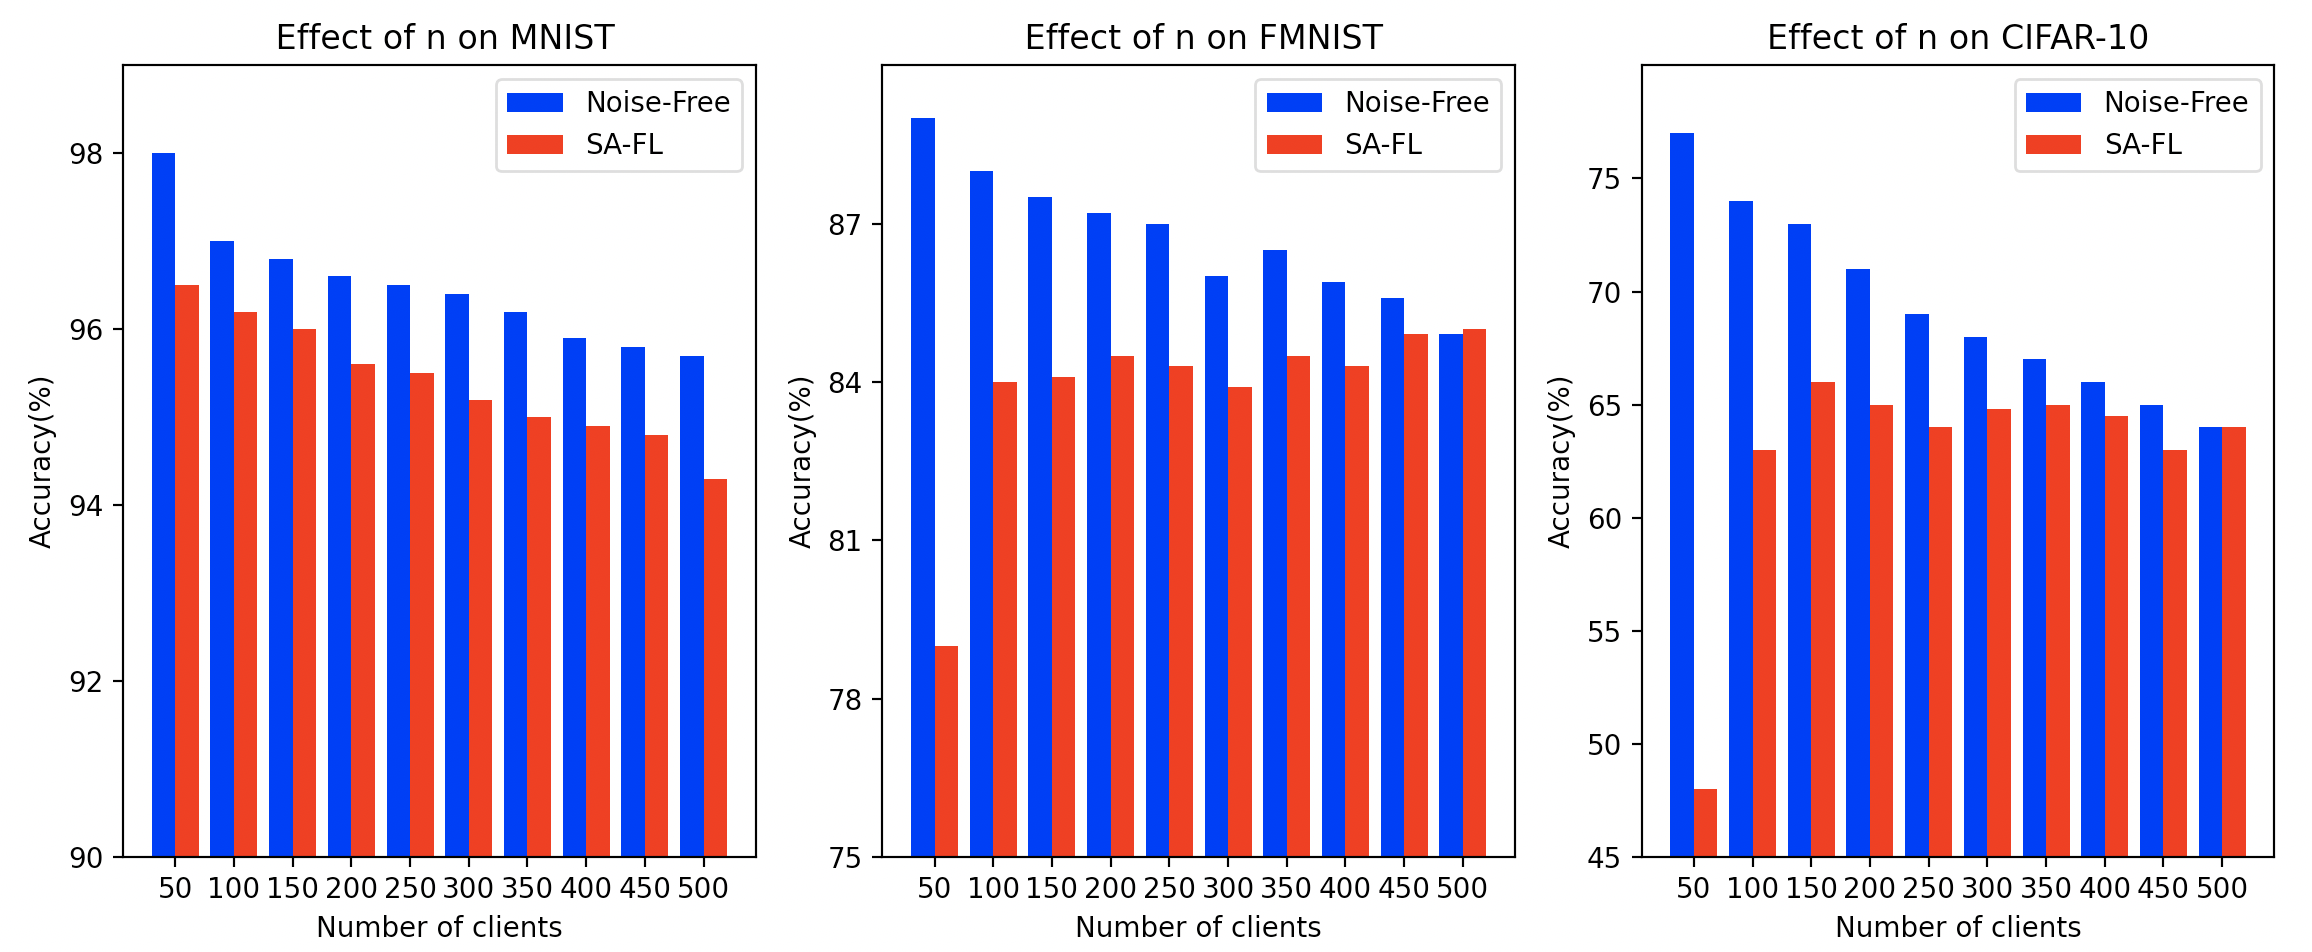
\includegraphics[scale=0.37]{fig2/C4/SA-FL1}%联邦学习的系统架构
	\caption{安全混洗模型中本地客户端数量对联邦学习模型训练精度的影响}
  	\label{fig:安全混洗模型中参与混洗的本地客户端数量对联合模型精度的影响} 
\end{figure}

如图\ref{fig:安全混洗模型中客户端采样比对联邦学习模型精度的影响}所示,当固定总客户端数量为100,在不同的隐私预算参数$\epsilon$=50、70、100和不添加隐私保护的联邦学习模型中,混洗器在每次迭代过程中随机采样部分客户端的梯度进行混洗。图\ref{fig:安全混洗模型中客户端采样比对联邦学习模型精度的影响}展示了全局损失函数值随客户端采样比的变化情况,总体来说,当客户端采样比为0.5左右时,损失函数值最小。联邦学习的隐私保护难点在于使用较低的隐私预算维持较高的模型精度,而选择适宜的客户端数量参与安全聚合会大大提升模型的收敛速度和通信性能。

\begin{figure}[!hbt]
\centering
  	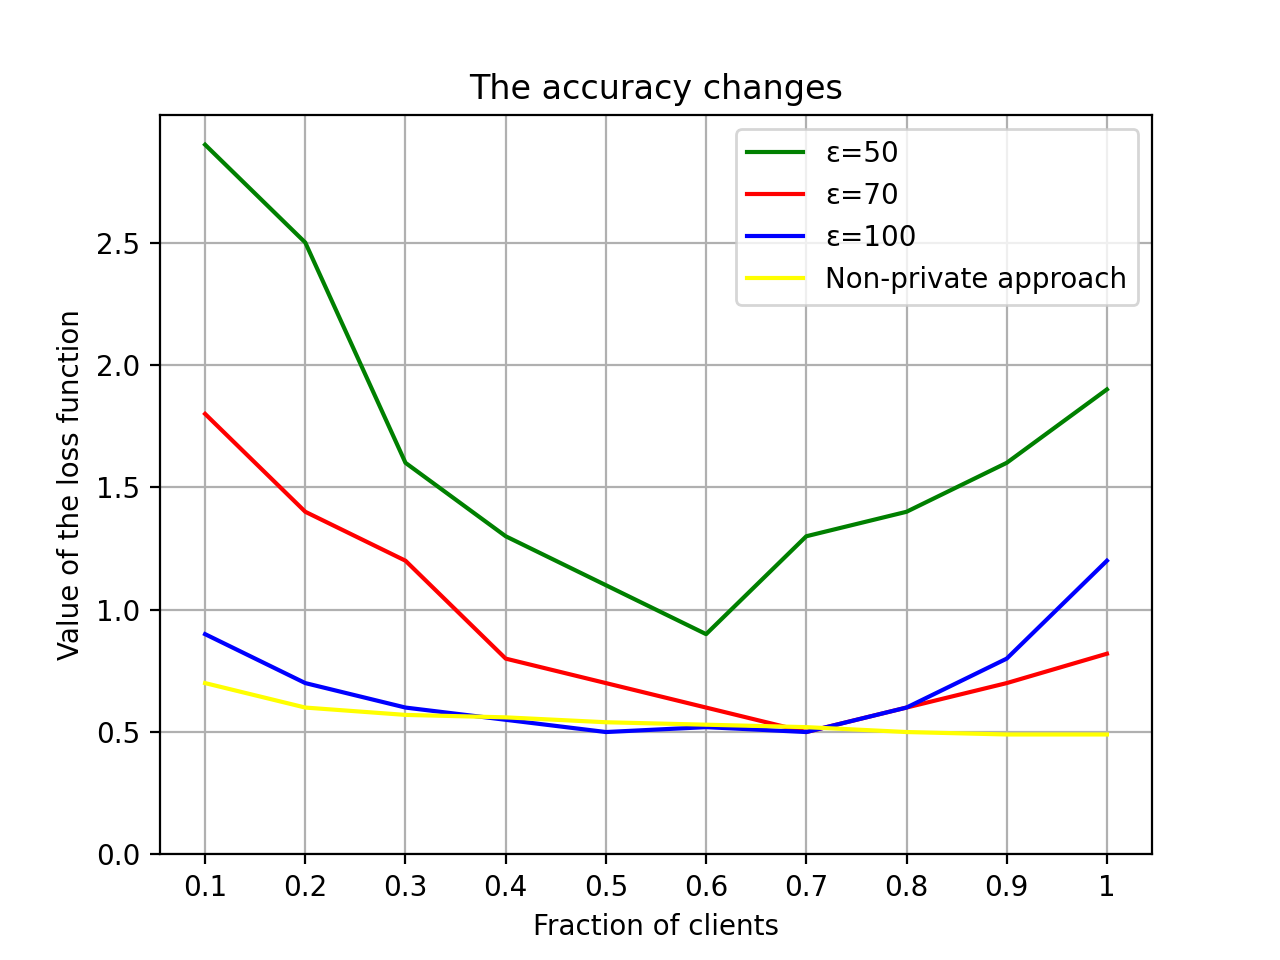
\includegraphics[scale=0.6]{fig2/C4/实验一客户端采样比}%联邦学习的系统架构
	\caption{安全混洗模型中客户端采样比对联邦学习模型训练精度的影响}
  	\label{fig:安全混洗模型中客户端采样比对联邦学习模型精度的影响} 
\end{figure}

\begin{figure}[!hbt]
\centering
  	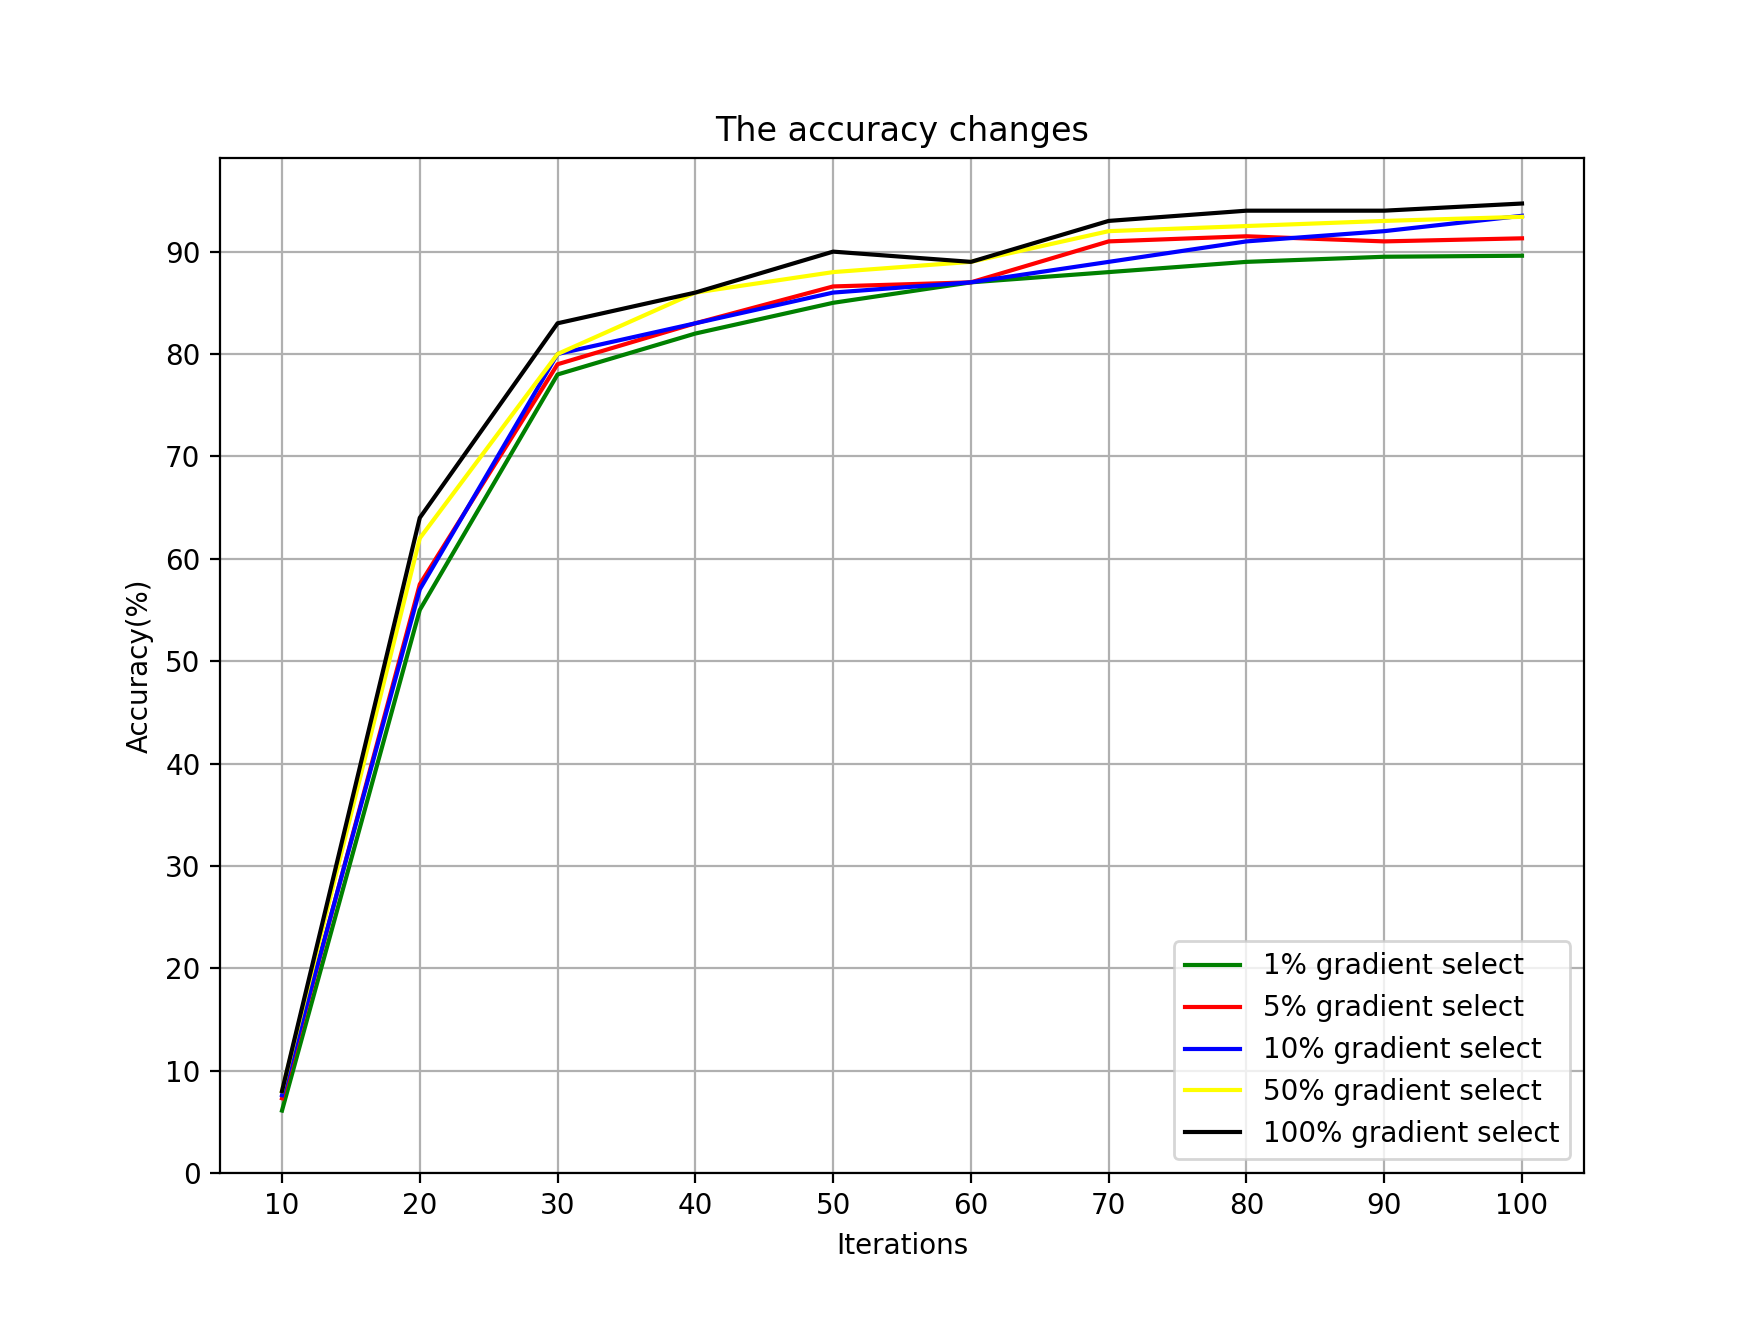
\includegraphics[scale=0.5]{fig2/C4/实验一K值}%联邦学习的系统架构
	\caption{安全混洗模型中梯度选择比率对联邦学习模型训练精度的影响}
  	\label{fig:安全混洗模型中梯度选择比率对联邦学习模型训练精度的影响} 
\end{figure}

如图\ref{fig:安全混洗模型中梯度选择比率对联邦学习模型训练精度的影响}展示了不同的梯度选择比率对联邦学习模型训练精度的影响,X轴表示联邦模型迭代次数。从图中的曲线变化情况可以看出,各个梯度选择比率的模型收敛速度接近,在70个训练回合后基本达到收敛,因此梯度选择并不会影响模型的收敛速度。1\%的梯度选择在历时100个训练回合后能达到83\%的准确率,100\%的梯度选择比率所能达到的模型准确率为95\%,相差了近10\%的准确率,可见部分梯度的丢弃确实丢失了部分的训练信息。当梯度选择比率低于10\%时,随着梯度选择比率的增加,模型的准确率也增加了接近3\%-5\%个百分点,然而当梯度选择比率为50\%时,模型在30个训练回合后的准确率基本与100\%的梯度选择比率所能达到的模型准确率接近。

在实验中,每一轮的迭代训练都需要由中央服务器和本地客户端交互计算,我们分别计算了不同的梯度选择比率在一次训练迭代中的通信开销,实验结果如表\ref{不同梯度选择比率的通信开销}所示。当梯度选择比率下降时,通信开销也基本呈比例下降。当Top-K梯度选择比率从100\%优化至50\%时,通信性能优化了大约1.99倍,而根据图\ref{fig:安全混洗模型中梯度选择比率对联邦学习模型训练精度的影响}所示,在梯度选择比率从100\%降低至50\%时,模型的训练准确率并不会受到太大影响,由此可见一定范围内的梯度选择可以较好的优化联邦学习模型的通信性能。

\begin{table}[H]
	\centering
	\begin{tabular}{cc}
		\hline
		Top-K/\%& 通信开销/KB\\
		\hline
		1& 167.022×2\\
		5& 863.317×2\\
		10& 1684.271×2\\
		50& 3502.151×2\\
		100& 6995.548×2\\
		\hline
	\end{tabular}
	\caption{不同梯度选择比率的通信开销}
	\label{不同梯度选择比率的通信开销}
\end{table}

\subsubsection{实验二(与前人的隐私保护方案进行对比实验)} 
我们将本文设计的基于梯度选择与安全混洗的联邦学习隐私保护方案(KSA-FL)的与FL、PS-FL、DP-FL、LDP-FL方案进行对比实验,选取的数据集为MNIST,网络模型为CNN5。我们比较了不同方案在给定相同的隐私预算($(0.2,5 \mathrm{e}-6)-\mathrm{DP}$)情况下,模型分类准确率变化情况。

\begin{figure}[!hbt]
\centering
  	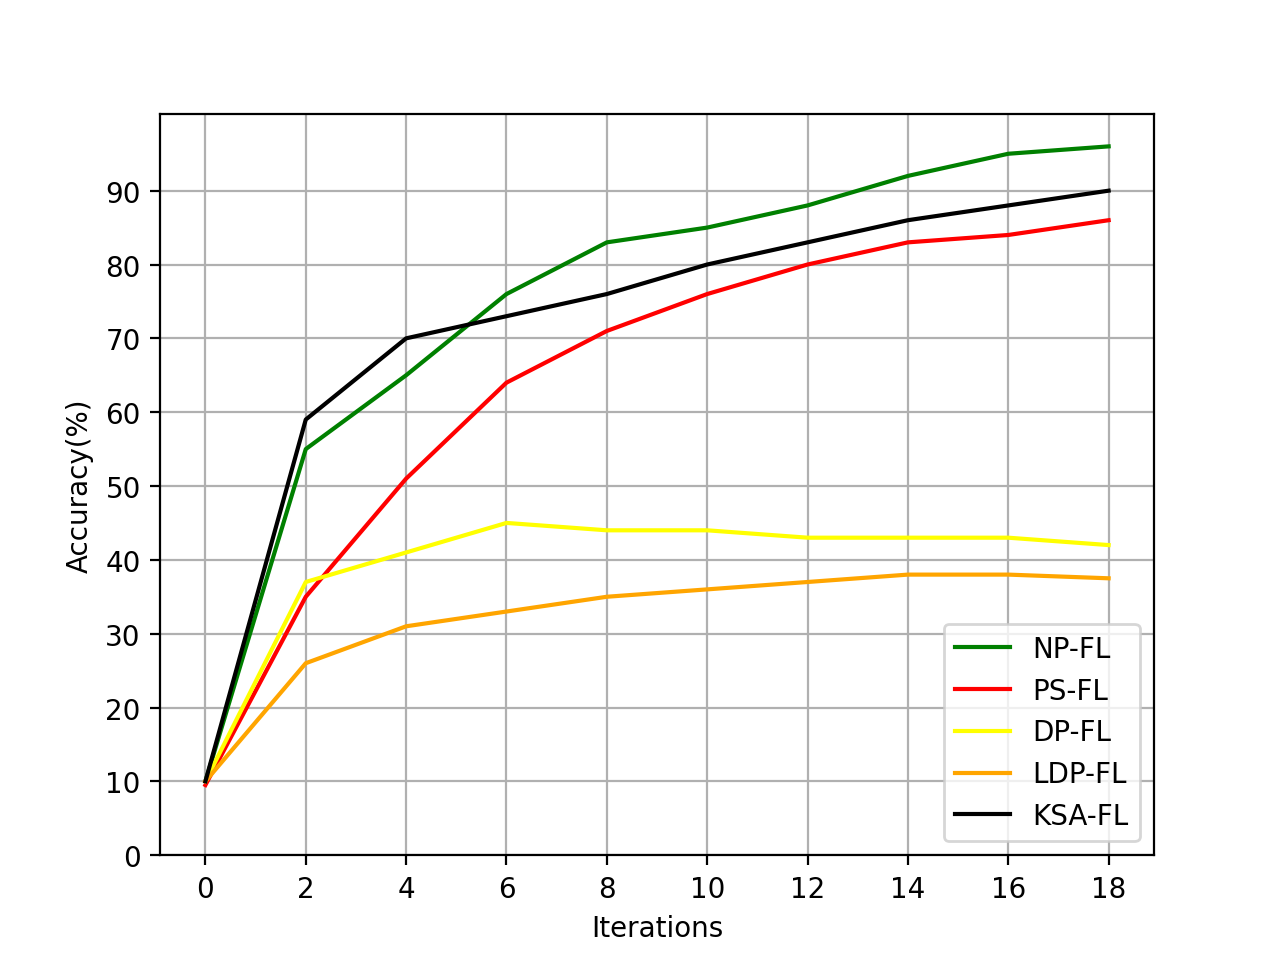
\includegraphics[scale=0.6]{fig2/C4/实验二}%联邦学习的系统架构
	\caption{不同隐私保护方案在MNIST数据集上训练的模型分类准确率变化情况}
  	\label{fig:不同隐私保护方案在MNIST数据集上训练的模型分类准确率变化情况} 
\end{figure}

在($(0.2,5 \mathrm{e}-6)-\mathrm{DP}$)的隐私预算下,无添加隐私保护的联邦学习基准模型在18个训练轮次后能达到94\%左右的准确率,其余四种实现了联邦学习隐私保护的方案中,本文所设计的Top-K安全混洗方案所能达到的准确率最高,在18个训练轮次后能达到90\%的准确率,而在训练开始阶段,模型的准确率提升速度甚至超过了无添加隐私保护的联邦学习基准模型,这表明Top-K梯度选择算法能有效的加速模型的学习速率。基于中央差分隐私的联邦学习隐私保护模型在18个训练轮次后能达到41\%左右的准确率,在6个训练轮次过后,模型就接近收敛。基于本地差分隐私的联邦学习隐私保护模型的分类准确率在这几种方案中的表现最低,正如上文分析的,本地差分隐私由于局部噪声带来的误差会随着维度系数的增加而加剧,从而大大降低模型的精度。

\subsubsection{实验三(针对攻击模型,分析该方案的隐私保护效用)} 

\section{本章总结}
本章节我们针对联邦学习模型的整体框架进行了改进,提出了安全混洗模型,在本地客户端和中央服务器之间加设混洗器,通过对本地客户端进行随机抽样,将上传的梯度进行拆分混洗,增加隐私放大效果。然后发送给中央服务器进行聚合。并对方案进行了隐私性证明,表明此安全混洗算法可以保证$\varepsilon_{\mathrm{c}}$差分隐私,然后对此方案在中央服务器上的随机梯度下降算法进行了收敛性的分析,证明在凸函数上,梯度$\mathbf{g}_{t}$满足$\mathbb{E}\left[\mathbf{g}_{t}\right]=\nabla_{\theta_{t}} F\left(\theta_{t}\right)$时模型能达到全局收敛。最后,通过在三种基准数据集上进行对象,证明本章所提出的方案能在保证模型收敛性的情况下,减少隐私预算。


